%%%%%%%%%%%%%%%%%%%%%%%%%%%%%%%%%%%%%%%%%
% Beamer Presentation
% LaTeX Template
% Version 1.0 (10/11/12)
%
% This template has been downloaded from:
% http://www.LaTeXTemplates.com
%
% License:
% CC BY-NC-SA 3.0 (http://creativecommons.org/licenses/by-nc-sa/3.0/)
%
%%%%%%%%%%%%%%%%%%%%%%%%%%%%%%%%%%%%%%%%%

%----------------------------------------------------------------------------------------
%	PACKAGES AND THEMES
%----------------------------------------------------------------------------------------

\documentclass[aspectratio=169]{beamer}
\usepackage[utf8]{inputenc}
\usepackage{booktabs}
\usepackage{graphicx}
\usepackage{array}
\usepackage{caption}
\usepackage{threeparttable}
\usepackage{lscape}
\usepackage{import}
\usepackage{amsmath}
\usepackage{csvsimple}
\usepackage{siunitx}
\usepackage{subfigure}
\usepackage{filecontents}
\newenvironment{wideitemize}{\itemize\addtolength{\itemsep}{10pt}}{\enditemize}
\usepackage{appendixnumberbeamer}
\usepackage{float}
\usepackage{amsmath}  
\usepackage{tikz,pgfplots}
\usepackage{tkz-fct}
\usepackage{amsthm}
\pgfplotsset{compat=1.10}
\usepgfplotslibrary{fillbetween}
\newcommand{\vertLineFromPoint}[1]{
  \draw[dashed] 
  (#1) -- (#1|-{rel axis cs:0,0})
}
\newcommand{\horLineFromPoint}[1]{
  \draw[dashed] 
  (#1) -- (#1-|{rel axis cs:0,0})
}
\mode<presentation> {
\AtBeginSection[]
{
    \begin{frame}
        \frametitle{Table of Contents}
        \tableofcontents[currentsection]
    \end{frame}
}

% The Beamer class comes with a number of default slide themes
% which change the colors and layouts of slides. Below this is a list
% of all the themes, uncomment each in turn to see what they look like.

%\usetheme{default}
%\usetheme{AnnArbor}
%\usetheme{Antibes} -
%\usetheme{Bergen}
%\usetheme{Berkeley}
%\usetheme{Berlin}
\usetheme{Boadilla}
%\usetheme{CambridgeUS}
%\usetheme{Copenhagen} -
%\usetheme{Darmstadt}
%\usetheme{Dresden}
%\usetheme{Frankfurt}
%\usetheme{Goettingen}
%\usetheme{Hannover}
%\usetheme{Ilmenau}
%\usetheme{JuanLesPins}
%\usetheme{Luebeck}
%\usetheme{Madrid}
%\usetheme{Malmoe}
%\usetheme{Marburg}
%\usetheme{Montpellier}
%\usetheme{PaloAlto}
%\usetheme{Pittsburgh}
%\usetheme{Rochester} -
%\usetheme{Singapore}
%\usetheme{Szeged}
%\usetheme{Warsaw}

% As well as themes, the Beamer class has a number of color themes
% for any slide theme. Uncomment each of these in turn to see how it
% changes the colors of your current slide theme.

%\usecolortheme{albatross}
%\usecolortheme{beaver}
%\usecolortheme{beetle}
%\usecolortheme{crane}
%\usecolortheme{dolphin}
%\usecolortheme{dove}
%\usecolortheme{fly}
%\usecolortheme{lily}
%\usecolortheme{orchid}
%\usecolortheme{rose}
%\usecolortheme{seagull}
%\usecolortheme{seahorse}
%\usecolortheme{whale}
%\usecolortheme{wolverine}

%\setbeamertemplate{footline} % To remove the footer line in all slides uncomment this line
\setbeamertemplate{footline}[frame number] % To replace the footer line in all slides with a simple slide count uncomment this line
\setbeamertemplate{theorems}[numbered]
\setbeamertemplate{navigation symbols}{} % To remove the navigation symbols from the bottom of all slides uncomment this line
}
\setbeamertemplate{caption}{\raggedright\insertcaption\par}
  \setbeamertemplate{enumerate items}[default]
\usepackage{graphicx} % Allows including images
\usepackage{booktabs} % Allows the use of \toprule, \midrule and \bottomrule in tables
%\usepackage {tikz}
\newtheorem*{theorem*}{Theorem}
\newtheorem*{lemma*}{Lemma}
\newtheorem*{proposition}{Proposition}
\newtheorem*{corollary*}{Corollary}
\newtheorem*{definition*}{Definition}
\DeclareMathOperator*{\argmin}{arg\,min}
\newtheorem*{assumption}{Assumption}
\usetikzlibrary {positioning}
% macro for inputting terminal nodes
\newcommand\term[2]{\node[below]at(#1){$#2$};}
%
%\usepackage {xcolor}

%----------------------------------------------------------------------------------------
%	TITLE PAGE
%----------------------------------------------------------------------------------------

\title[Spatial]{Lecture 6: Sequential Games} % The short title appears at the bottom of every slide, the full title is only on the title page

\author{Jacob Kohlhepp} % Your name
\institute[UCLA] % Your institution as it will appear on the bottom of every slide, may be shorthand to save space
{
Econ 101 \\ % Your institution for the title page
\medskip
}
\date{\today} % Date, can be changed to a custom date

\begin{document}

\begin{frame}
\titlepage % Print the title page as the first slide
\end{frame}

\begin{frame}{Introduction}
\begin{wideitemize}
    \item In many economic situations, people move \textbf{sequentially}, taking into account prior actions.
    \item This introduces more strategic effects.
    \item To analyze these situations we need to broaden our tool set.
    \item After this lecture you should be able to solve finite dynamic games (those where $1<T<\infty$).
    \item Next class we will learn to solve infinite repeated games (the same game is played over and over forever).
\end{wideitemize}
\end{frame}

\begin{frame}{Entry Example}
Consider the following game:
\begin{wideitemize}
    \item At $t=1$ Firm A decides whether to enter the market for designer jeans at fixed cost $4$.
    \item Firm B is a long time producer of jeans. At $t=2$, Firm B can choose to flood the market with jeans or not.
    \item If Firm A does not enter, it makes 0 profit regardless of what Firm B does.
    \item If Firm B floods, profit for all entrants is $3$ less the entry cost for A. 
    
    \item If Firm B does not flood profit is $6$ if firm A enters and $10$ otherwise, (less any entry costs for firm A).
    \item Notice that the strategy of firm B depends on the entry decision. It is no longer an action but a function!
\end{wideitemize}
    
\end{frame}

\begin{frame}{Entry Example}
This is a lot to track. We can summarize it in a  game tree:

\begin{tikzpicture}[scale=1.5,font=\footnotesize]
\tikzstyle{solid node}=[circle,draw,inner sep=1.5,fill=black]
\tikzstyle{hollow node}=[circle,draw,inner sep=1.5]
\tikzstyle{level 1}=[level distance=15mm,sibling distance=3.5cm]
\tikzstyle{level 2}=[level distance=15mm,sibling distance=1.5cm]
\tikzstyle{level 3}=[level distance=15mm,sibling distance=1cm]
\node(0)[solid node,label=above:{$A$}]{}
child{node[solid node,label=above left:{$B$}]{}
child{node[hollow node,label=below:{$(0,3)$}]{} edge from parent node[left]{$flood$}}
child{node[hollow node,label=below:{$(0,10)$}]{} edge from parent node[right]{$not$}}
edge from parent node[left,xshift=-5]{$not$}
}
child{node[solid node,label=above left:{$B$}]{}
child{node[hollow node,label=below:{$(-1,3)$}]{} edge from parent node[left]{$flood$}}
child{node[hollow node,label=below:{$(2,6)$}]{} edge from parent node[right]{$not$}}
edge from parent node[left,xshift=-5]{$enter$}
};
\end{tikzpicture}
\end{frame}
\begin{frame}{Finding Two NE}
    See handwritten notes.
\end{frame}
\begin{frame}{Refining Nash Equilibrium}
    \begin{wideitemize}
        \item One NE we derived consists of a \textbf{non-credible threat.}
        \item Given that Firm A has already entered, Firm B has no reason to follow through on flooding.
        \item We need a new equilibrium concept that removes such irrational equilibria.
        \item First we need a new definition.
        \begin{definition}
    A \textbf{proper subgame} is a part of the extensive form beginning at a decision node that is not part of an information set and including everything that branches down from it.
    \end{definition}
    \end{wideitemize}
\end{frame}

\begin{frame}{Entry Example}{Identifying Subgames}
\begin{tikzpicture}[scale=1.5,font=\footnotesize]
\tikzstyle{solid node}=[circle,draw,inner sep=1.5,fill=black]
\tikzstyle{hollow node}=[circle,draw,inner sep=1.5]
\tikzstyle{level 1}=[level distance=15mm,sibling distance=3.5cm]
\tikzstyle{level 2}=[level distance=15mm,sibling distance=1.5cm]
\tikzstyle{level 3}=[level distance=15mm,sibling distance=1cm]
\node(0)[solid node,label=above:{$A$}]{}
child{node[solid node,label=above left:{$B$}]{}
child{node[hollow node,label=below:{$(0,6)$}]{} edge from parent node[left]{$flood$}}
child{node[hollow node,label=below:{$(0,10)$}]{} edge from parent node[right]{$not$}}
edge from parent node[left,xshift=-5]{$not$}
}
child{node[solid node,label=above left:{$B$}]{}
child{node[hollow node,label=below:{$(-1,3)$}]{} edge from parent node[left]{$flood$}}
child{node[hollow node,label=below:{$(2,6)$}]{} edge from parent node[right]{$not$}}
edge from parent node[left,xshift=-5]{$enter$}
};
\end{tikzpicture}
\end{frame}

\begin{frame}{Subgame Perfect Nash Equilibrium}

\begin{wideitemize}
    \item Armed with our definition of a subgame, we can define a new equilibrium concept:
    \begin{definition}
    A \textbf{subgame-perfect Nash Equilibrium} (SPNE) is a strategy profile $(s_1^*,...,s_n^*)$ that is a Nash equilibrium in every proper subgame.
    \end{definition}
    \item All SPNE are NE, not all NE are SPNE!
    \item We can find SPNE using backwards induction.
\end{wideitemize}
    
\end{frame}

\begin{frame}{Entry Example}{Demonstrating Backwards Induction}

\begin{tikzpicture}[scale=1.5,font=\footnotesize]
\tikzstyle{solid node}=[circle,draw,inner sep=1.5,fill=black]
\tikzstyle{hollow node}=[circle,draw,inner sep=1.5]
\tikzstyle{level 1}=[level distance=15mm,sibling distance=3.5cm]
\tikzstyle{level 2}=[level distance=15mm,sibling distance=1.5cm]
\tikzstyle{level 3}=[level distance=15mm,sibling distance=1cm]
\node(0)[solid node,label=above:{$A$}]{}
child{node[solid node,label=above left:{$B$}]{}
child{node[hollow node,label=below:{$(0,6)$}]{} edge from parent node[left]{$flood$}}
child{node[hollow node,label=below:{$(0,10)$}]{} edge from parent node[right]{$not$}}
edge from parent node[left,xshift=-5]{$not$}
}
child{node[solid node,label=above left:{$B$}]{}
child{node[hollow node,label=below:{$(-1,3)$}]{} edge from parent node[left]{$flood$}}
child{node[hollow node,label=below:{$(2,6)$}]{} edge from parent node[right]{$not$}}
edge from parent node[left,xshift=-5]{$enter$}
};
\end{tikzpicture}
\end{frame}


\begin{frame}{The Pirate Riddle}
There is a very famous and tricky riddle that you can solve using SPNE. We will use it to practice backwards induction.
\begin{quote}
    Five pirates, numbered 1 through 5, must decide how to divide 100 gold coins. Their decision process is as follows. Starting with pirate 1, each pirate proposes a split consisting of a number of coins for each of the pirates on the ship. Then all pirates vote. If a strict majority approve, the allocation happens. If it does not the proposer is thrown off the ship and the remaining pirates repeat the process. Assume pirates value 2 coins more than 1, etc and that getting thrown off is worse than getting 0 coins. Assume pirates vote no when indifferent (they get a little bit of enjoyment from watching someone walk the plank). What is the maximum number of coins P1 can obtain and not get thrown off?
\end{quote}
    
\end{frame}


\begin{frame}{Pirate Riddle: Verbal Solution}

\begin{wideitemize}
    \item Start from the end of the game. If P5 gets to make a proposal, then they are the last pirate left. They propose 100 coins for themselves and get it!\pause
    \item Rolling back, P4 needs pirate 5's vote for a strict majority. There is no way to get it since P5 knows they get 100 coins if they throw off 4. Thus P4 can propose anything, and P5 always rejects.\pause
    \item Roll back. P3 needs 1 other vote to get a majority. The easiest person to convince is pirate 4, since pirate 4 gets thrown off if the game continues. To get P4's vote P3 can get away with giving him/her 0 coins. P3 proposes\pause
    \item Roll back. Pirate 2 needs to get two votes. P4 and P5 are the cheapest to convince because they get 0 next round. So P2 gives P4 and P5 1, P3 0, and keeps 98.\pause
    \item Roll back. P1 needs two other votes. P3 is the cheapest to convince. P4 and P5 are next cheapest, and P1 need only convince one. So P1 proposes 0 for P2 and P5, P3 1, and P4 2 and keeps 97!\pause
\end{wideitemize}
\end{frame}

\begin{frame}{Interpreting the Pirate Game}
\begin{wideitemize}
    \item Brief comment on SPNE vs outcome (see lecture recording).
    \item Despite the fact that all pirates are identical with equal voting power, the first player gets 97 out of 100 coins.
    \item There is a first mover advantage: going first gives a higher payoff.
    \item This advantage exists in many games, including bargaining and in Stackleberg model (see problem set).
    \item Because voting is involved, this also illustrates \textbf{agenda setting power.}
    \item The ability to decide what gets considered first is very valuable.
    \item Examples: Congress, corporate board meetings, etc.
    
\end{wideitemize}

    
\end{frame}

\begin{frame}{Interpreting the Pirate Game, Meta Discussion}
    \begin{columns}[T] % align columns
\begin{column}{.63\textwidth}
    \begin{wideitemize}
        \item Models are just stylized stories that help us understand the world.
        \item They can be unreasonable! Assuming this degree of rationality and forward looking behavior is a little silly (especially for pirates).
        \item Indeed, Kalah (from ancient African game mancala), is solved: the first player can always win if they play optimally!
        \item But people play as if the game is not determined! Why?
        \item Extreme example: Chess. Finite moves, not solved!
    \end{wideitemize}
\end{column}%
\hfill%
\begin{column}{.34\textwidth}
\vspace{20mm}
\resizebox{\textwidth}{!}{
  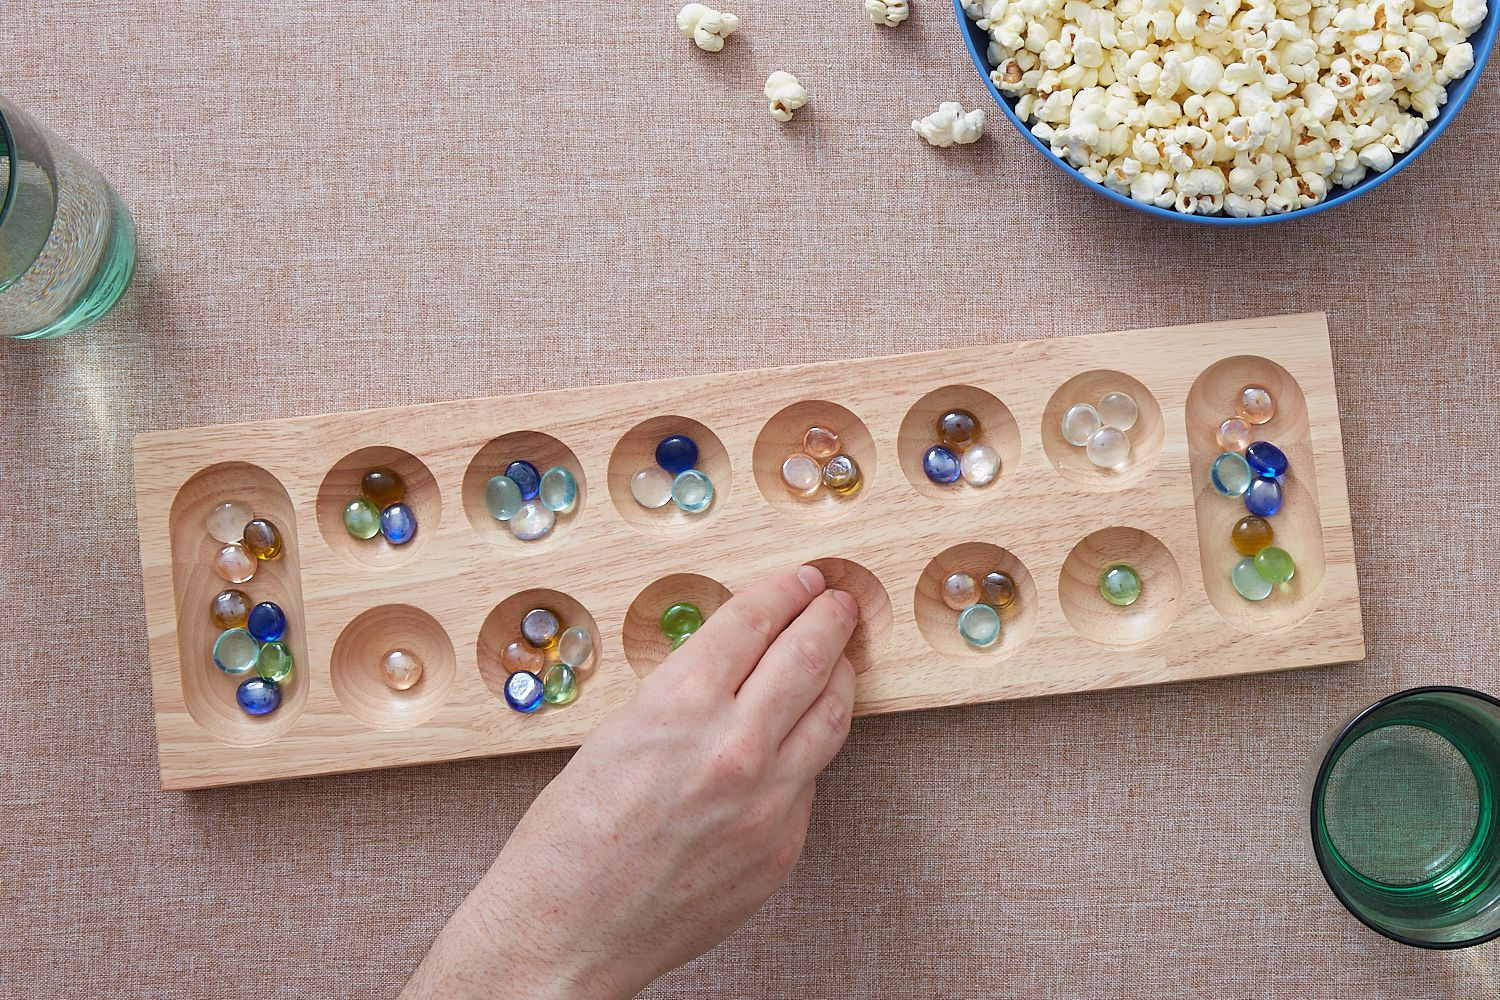
\includegraphics{how-to-win-at-mancala-basic-strategy-411832_hero_2873-1e7293a6034e4dbf9d563cd94ed2915c.jpg}
}

  \hfill Source: The Spruce Crafts
\end{column}%
\end{columns}
\end{frame}

\begin{frame}{Another Example: Investment as Commitment }
\begin{wideitemize}
    \item We now apply SPNE again to illustrate the value of commitment.
    \item Consider the entry game from earlier. Remember that the only SPNE was that firm A enters and firm B does not flood.
    \item Add a stage to the game before the entry decision: Firm B can invest in increased manufacturing capacity at cost $K$.
    \item If it does so, the payoff from flooding the market becomes 1 more than not flooding regardless of whether firm A enters.
    \item Find the SPNE based on $K$.
\end{wideitemize}
    
\end{frame}


\begin{frame}{Investment As Commitment}
\centering
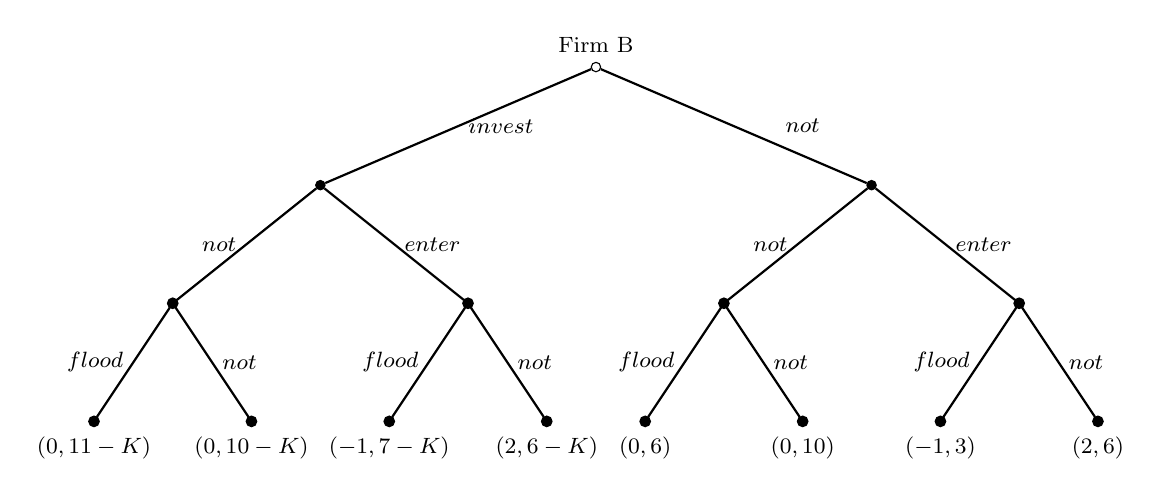
\begin{tikzpicture}[font=\footnotesize,edge from parent/.style={draw,thick}]
% Two node styles: solid and hollow
\tikzstyle{solid node}=[circle,draw,inner sep=1.2,fill=black];
\tikzstyle{hollow node}=[circle,draw,inner sep=1.2];
% Specify spacing for each level of the tree
\tikzstyle{level 1}=[level distance=15mm,sibling distance=7cm]
\tikzstyle{level 2}=[level distance=15mm,sibling distance=3.75cm]
\tikzstyle{level 3}=[level distance=15mm,sibling distance=2cm]
% The Tree
\node(0)[hollow node,label=above:{Firm B}]{}
child{node[solid node]{}
child{node[solid node]{}
child{node[solid node,label=below:{$(0,11-K)$}]{}edge from parent node[left]{$flood$}}
child{node[solid node,label=below:{$(0,10-K)$}]{}edge from parent node[right]{$not$}}
edge from parent node[left]{$not$}
}
child{node[solid node]{}
child{node[solid node,label=below:{$(-1,7-K)$}]{}edge from parent node[left]{$flood$}}
child{node[solid node,label=below:{$(2,6-K)$}]{}edge from parent node[right]{$not$}}
edge from parent node[right]{$enter$}
}
edge from parent node[right]{$invest$}
}
child[sibling distance=\tikzsiblingdistance]{node[solid node]{}
child{node[solid node]{}
child{node[solid node,label=below:{$(0,6)$}]{}edge from parent node[left]{$flood$}}
child{node[solid node,label=below:{$(0,10)$}]{}edge from parent node[right]{$not$}}
edge from parent node[left]{$not$}
}
child{node[solid node]{}
child{node[solid node,label=below:{$(-1,3)$}]{}edge from parent node[left]{$flood$}}
child{node[solid node,label=below:{$(2,6)$}]{}edge from parent node[right]{$not$}}
edge from parent node[right]{$enter$}
}
edge from parent node[right,xshift=15]{$not$}
};
% specifying terminal nodes
%\newcounter{tnode}
%\setcounter{tnode}{0}
%\term{0-1}{T_\arabic{tnode}}
%\foreach \x in {2,3}
%\foreach \y in {1,2}
%\foreach \z in {1,2}
%\stepcounter{tnode}
%\term{0-\x-\y-\z}{T_\arabic{tnode}};
\end{tikzpicture}
\end{frame}

\begin{frame}{Interpreting Investment as Commitment}
\begin{wideitemize}
    \item See handwritten notes for solution.
    \item The upfront investment \textbf{credibly commits} firm B to flood the market.
    \item This induces firm A to stay out.
    \item Thus this is a form of entry deterrence.
\end{wideitemize}
\end{frame}

\begin{frame}{Hotelling with Location Choice}
Recall the Hotelling product differentiation model from several classes ago.
\begin{wideitemize}
    \item In a simultaneous game where two hot dog stands set prices given fixed locations, we derived that prices were:
    \[p^*_A = \frac{t}{3} (b-a)(2L+a+b)\qquad p^*_B =\frac{t}{3} (b-a)(4L-a-b) \]
    \item This is in a static NE without location choice. Suppose now we add a first stage where firms simultaneously choose locations along the pier.
    \item That is firm A and B choose locations $a,b$ along the pier at $t=1$, then compete in prices given locations at $t=2$.
    \item Now we can utilize backwards induction and SPNE to understand equilibrium behavior.
\end{wideitemize}

\end{frame}
\begin{frame}{Hotelling with Location Choice: Solution}
    \begin{wideitemize}
        \item Treat locations as given in the price competition stage. This yields the solution we found last class:
        \[p^*_A = \frac{t}{3} (b-a)(2L+a+b)\qquad p^*_b =\frac{t}{3} (b-a)(4L-a-b)^2 \]
        \item The payoffs in the second stage with fixed locations are given by profit, which we also derived:
        \[\pi^*_A = \frac{t}{18} (b-a)(2L+a+b)^2 \qquad \pi^*_B = \frac{t}{18} (b-a)(4L-a-b)^2\]
        \item Now we can solve the location choice part of the game using profit as the objective to maximize. (See handwritten notes).
    \end{wideitemize}
\end{frame}

\begin{frame}{Hotelling with Location Choice: Solution}
    \begin{wideitemize}
        \item SPNE locations are:
        \[a^*=0, \qquad b^*=L\]
        \begin{definition}
        The \textbf{principle of maximum differentiation} refers to the idea that firms want to make their products as different as possible in order to minimize price competition.
        \end{definition}
        \item It can be shown that the socially optimal locations are $a^{**}=0.25 L, b^{**}=0.75L$.\footnote{Showing this requires showing that all that matters for social surplus is transport cost. It is a little involved so you are not required to derive it.}
        \item There is too much differentiation in equilibrium.
        
    \end{wideitemize}
\end{frame}

\begin{frame}{Interpretation of Hotelling with Location Choice}
\begin{wideitemize}
    \item In reality we often see instances where competing firms cluster together (gas stations, burger joints, etc).
    \item This is inconsistent with the previous model.
    \item However if we think price is fixed in the second round we get that $a^*=b^*=0.5L$.
    \begin{definition}
    The principle of \textbf{minimal differentiation} (Hotelling's Law) refers to the idea that absent price competition firms often want to make their products as similar as possible.
    \end{definition}
    \item This is also inefficient (by same argument as before). We have too little differentiation.
    \item Fixed prices represents electoral competition well: Downs applied the reduced Hotelling model to describe why political parties in the US tend to gravitate towards the center on issues (Median Voter Theorem).
    
\end{wideitemize}
    
\end{frame}
\end{document}

